\section{Durchführung}
\label{sec:Durchführung}

Die zu untersuchenden Materialien werden vor dem Versuch aktiviert.
Dafür müssen zunächst niederenergetische Neutronen erzeugt werden.
Dies geschieht durch den Beschuss von $\ce{^{9}Be}$-Kernen mit $\alpha$-Teilchen, welche bei dem Zerfall von $\ce{^{226}Ra}$-Kernen entstehen.
Die so entstehenden Neutronen müssen noch abgebremst werden.
Dafür durchqueren sie eine dicke Schicht aus Parafin.
Dies geschieht in einem abgeschirmten Behälter.
Um die Proben aktivieren zu können, stecken werden sie in geeigneten Bohrungen innerhalb des Parafins eingeführt.
Nach Ablaufen der Aktivierungszeit können die so aktivierten Proben dem Behälter entommen werden und in die Messvorrichtung eingeführt werden.
Der Aufbau der Messvorrichtung kann Abbildung \ref{fig:Aufbau} entnommen werden.

\begin{figure}
  \centering
  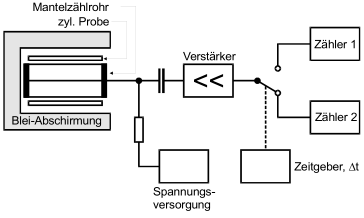
\includegraphics[width=0.5\textwidth]{images/Aufbau.png}
  \caption{Der Aufbau der verwendeten Messvorrichtung zur Bestimmung der Zerfallsereignisse pro Zeitintervall, entnommen der Versuchsanleitung \cite[8]{sample}.}
  \label{fig:Aufbau}
\end{figure}

Diese besteht aus einer Bleiabschirmung, einem Geiger-Müller-Zählrohr und einer Zählapparatur.
Die Probe wird in die Bleiabschirmung eingebracht und ummantelt das Geiger-Müller-Zählrohr.
Dieses misst einen konstanten Bruchteil der abgegebenen Strahlung.
Die ausgesendeten Signale werden verstärkt und auf eines von zwei Zählwerken geleitet.
Nach jeder Messung wird das Zählwerk gewechselt, so dass eine konstante Messung für mehrere hintereinanderfolgende Zeitintervalle gwährleistet wird.
Die Bleiabschirmung dientdazu den äußeren Strahlungseinfluss zu minimieren.
Damit dieser sogenannte Nulleffekt später berücksichtig werden kann, wird über $\SI{900}{\second}$ eine Messung ohne Probe durchgeführt.
Die Messzeiten für das Isotopengemisch von Silber $\ce{^{108}Ag}$ und $\ce{^{110}Ag}$, sowie für Indium $\ce{^{116}In}$ wurden im Vorfeld bestimmt.
Es ergibt sich für Indium eine Messzeit von $\SI{60}{\minute}$ mit Zeitintervallen von $\SI{4}{\minute}$.
Für Silber eine Messzeit von $\SI{7}{\minute}$ mit Zeitintervallen von $\SI{10}{\second}$.
Für jedes Zeitintervall werden die Counts notiert.
